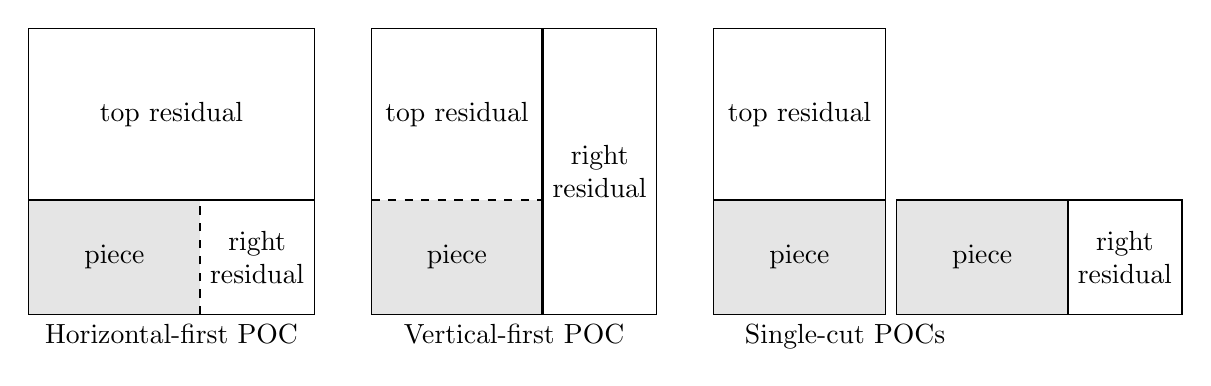
\begin{tikzpicture}[scale=0.145]
\def\piececolor{gray!20}
\def\labelxshift{12.5}
\def\labelyshift{0}
\def\labelfontsize{\normalsize}
\begin{scope}[shift={(0, 0)}] % FIRST ROW
\begin{scope}[shift={(0, 0)}] % FIRST IMAGE

\fill[\piececolor] (0, 0) rectangle +(15, 10);
\draw[thick, black] (0, 10) -- (25, 10);
\draw[dashed, thick, black] (15, 0) -- (15, 10);
\draw (0,0) rectangle +(25, 25);

\node [align=center, font=\labelfontsize\selectfont] at (7.5, 5) {\labelfontsize piece}; %{\labelfontsize piece-sized \\ \labelfontsize plate};
\node [align=center, font=\labelfontsize\selectfont] at (12.5, 17.5) {\labelfontsize top residual};
\node [align=center, font=\labelfontsize\selectfont] at (20, 5) {right\\residual};

\node [below] at (\labelxshift, \labelyshift) {\labelfontsize Horizontal-first POC};
\end{scope}

\begin{scope}[shift={(30, 0)}] % SECOND IMAGE

\fill[\piececolor] (0, 0) rectangle +(15, 10);
\draw[dashed, thick, black] (0, 10) -- (15, 10);
\draw[thick, black] (15, 0) -- (15, 25);
\draw (0,0) rectangle +(25, 25);

\node [align=center, font=\labelfontsize\selectfont] at (7.5, 5) {\labelfontsize piece}; %{\labelfontsize piece-sized \\ \labelfontsize plate};
\node [align=center, font=\labelfontsize\selectfont] at (7.5, 17.5) {\labelfontsize top residual};
\node [align=center, font=\labelfontsize\selectfont] at (20, 12.5) {right\\residual};

\node [below] at (\labelxshift, \labelyshift) {\labelfontsize Vertical-first POC};
\end{scope}

\begin{scope}[shift={(60, 0)}] % THIRD IMAGE

\fill[\piececolor] (0, 0) rectangle +(15, 10);
\draw[thick, black] (0, 10) -- (15, 10);
%\draw[dashed, thick, black] (15, 0) -- (15, 10);
\draw (0,0) rectangle +(15, 25);

\node [align=center, font=\labelfontsize\selectfont] at (7.5, 5) {\labelfontsize piece}; %{\labelfontsize piece-sized \\ \labelfontsize plate};
\node [align=center, font=\labelfontsize\selectfont] at (7.5, 17.5) {\labelfontsize top residual};
\end{scope}

\begin{scope}[shift={(76, 0)}] % FOURTH IMAGE

\fill[\piececolor] (0, 0) rectangle +(15, 10);
%\draw[dashed, thick, black] (0, 10) -- (15, 10);
\draw[thick, black] (15, 0) -- (15, 10);
\draw (0,0) rectangle +(25, 10);

\node [align=center, font=\labelfontsize\selectfont] at (7.5, 5) {\labelfontsize piece}; %{\labelfontsize piece-sized \\ \labelfontsize plate};
\node [align=center, font=\labelfontsize\selectfont] at (20, 5) {right\\residual};
\end{scope}
\node [below, align=center, font=\labelfontsize\selectfont] at (71.5, 0) {\labelfontsize Single-cut POCs};

\end{scope}
\end{tikzpicture}
